\label{egzakt}
A Green-függvény név indokolt: a teljességi reláció beszúrásával látható, hogy a kvantummechanikai Green-függény megegyezik a differenciálegyenletek elméletéből ismert Green-függvénnyel.
\begin{equation}
    \left(E-\op{H}\right)\op{G}\left( E \right) = \op{I},
\end{equation}
azaz
\begin{equation}
    \int dx^\prime \Bra{x}\left(E-\op{H}\right) \Ket{x^\prime}\Bra{x^\prime} \op{G}\left( E \right)\Ket{y} = \Bra{x}\op{I}\Ket{y} = \delta \left(x - y\right).
\end{equation} 
A $\Bra{x}\left(E-\op{H}\right) \Ket{x^\prime}$ maggal vett konvolúció az $E-\op{H}$ operátor hatása, ezért
\begin{equation}
    \left(E-\op{H}_x\right) G\left(x, y; E\right) = \delta\left(x - y\right),
\end{equation}
amely a differenciálegyenletek elméletéből ismert Green-függvény definíciója. Ebben a konkrét esetben
\begin{equation}
    \left(E +\frac{\hbar^2}{2m}\frac{\partial^2}{\partial x^2} - Fx \right) G\left(x, y; E\right) = \delta\left(x - y\right),
	\label{green:deltaeq}
\end{equation}
amely azt jelenti, hogy az $x < y$ tartományban, illetve $y < x$ tartományban a Green-függvény a homogén egyenlet megoldása. A homogén megoldások illesztését az eredeti differenciálegyenlet határfeltételei, valamint az $x = y$ pontban \aeqref{green:deltaeq} egyenlet $y$ körüli integrálásából kapott feltételek határozzák meg. A doboz falára vonatkozó határfeltételek
\begin{equation}
	\left. G\left(x,y;E\right)\right\rvert_{x = 0} = 0,
	\label{green:01}
\end{equation}
\begin{equation}
	\left. G\left(x,y;E\right)\right\rvert_{x = L} = 0.
	\label{green:02}
\end{equation}
\Aref{green:deltaeq}. egyenlet $x$ szerinti integrálja $y$ körüli $\epsilon$ sugarú környezetében az $\epsilon \to 0^+$ határesetben
\begin{equation}
	\lim_{\epsilon \to 0^+}\left.\frac{\partial}{\partial x}G\left(x,y;E \right)\right\rvert_{x = y - \epsilon}^{x = y + \epsilon} = \frac{2m}{\hbar^2}.
	\label{egzakt:jump}
\end{equation}
Itt a jobb oldal integrálja $\left. \theta\left(x - y\right) \right\rvert_{x = y - \epsilon}^{x = y + \epsilon} = 1$ az előírt határesetben. Mivel $G(x,y;E)$-ről feltesszük, hogy folytonos, a bal oldal integrálja is folytonos, leszámítva a deriváltakat tartalmazó tagokat. A határeset elvégzése közben a deriváltakat nem tartalmazó tagok így kiesnek. \Aref{green:deltaeq}. egyenlet $\int_{y-\epsilon}^{y+\epsilon}dx^\prime \int_{y-\epsilon}^{x^\prime} \,dx$ integrálja az $\epsilon \to 0^+$ határesetben
\begin{equation}
	\lim_{\epsilon \to 0^+}\left.G\left(x,y;E \right)\right\rvert_{x = y - \epsilon}^{x = y + \epsilon} = 0
	\label{green:continuity}
\end{equation}
folytonossági feltételt adja. A jobb oldal integrálja $\left. \left(x - y\right) \theta\left(x - y\right) \right\rvert_{x=y-\epsilon}^{x=y+\epsilon}$, ami a határesetben $0$. Az $\left(Fx - E\right)G\left(x,y;E\right)$ integrálja is $0$ a határesetben, az előző integrálhoz hasonló módon.

Valós energiákra $G(x,y;E)=G(y,x;E)^*$. Ezt a szimmetria tulajdonságot fel lehet használni a Green-függvényre adott ansatz pontosítására az $x<y$ és $y<x$ $x$-$y$ csere szimmetriájának megkövetelésével. Ez automatikusan kielégíti \aeqref{green:continuity} egyenletet. A tartomány peremén a homogén megoldás eltűnését megkövetelve \aeqref{green:01} és \aeqref{green:02} teljesül. Érdemes bevezetni a
\begin{equation}
	\begin{aligned}
		u &= ax-bE,
		v &= ay-bE
	\end{aligned}
	\label{egzakt:uv}
\end{equation}
jelöléseket. A fent leírt három kritériumot és szimmetria tulajdonságot teljesítő ansatz a
\begin{equation}
	G\left(x,y;E\right) = C_0(E)\times
	\begin{cases}
		\begin{split}
			\Bigl(\Ti(aL-bE)\Bi(v)-\Ai(v)\Bigr)\times\\
			\Bigl(\Ti(-bE)\Bi(u)-\Ai(u)\Bigr)
		\end{split}& x \leq y\\
		\begin{split}
			\Bigl(\Ti(aL-bE)\Bi(u)-\Ai(u)\Bigr)\times\\
			\Bigl(\Ti(-bE)\Bi(v)-\Ai(v)\Bigr)
		\end{split}& x \geq y
	\end{cases}.
	\label{egzakt:ansatz}
\end{equation}
A $C_0(E)$ együtthatót úgy kell megválasztani, hogy \aeqref{egzakt:jump} egyenlet teljesüljön. \Aeqref{egzakt:jump} egyenletbe behelyettesítve \aeqref{egzakt:ansatz} egyenlet, és osztva $C_0(E)$-vel,
\begin{dmath}
	\frac{1}{C_0(E)}\frac{2m}{\hbar^2}=\frac{1}{C_0(E)}\lim_{\epsilon \to 0^+}\left.\frac{\partial G(x,y;E)}{\partial x}\right\rvert_{x=y-\epsilon}^{x=y+\epsilon}=a\lim_{\epsilon \to 0^+}\Bigl(-\Ti(aL-bE)\Bip(u)\Ai(v)-\Ti(-bE)\Aip(u)\Bi(v)+\Ti(aL-bE)\Bi(v)\Aip(u)+\Ti(-bE)\Ai(v)\Bip(u)\Bigr)=a\Bigl(\Ti(-bE)-\Ti(aL-bE)\Bigr)\Bigl(\Ai(v)\Bip(v)-\Aip(v)\Bi(v)\Bigr)=a\frac{\Ti(-bE)-\Ti(aL-bE)}{\pi}.
	\label{egzakt:c0calc}
\end{dmath}
A második egyenlőségnél kihasználtuk, hogy a $\Bi(v)\Bip(u)$-t és $\Ai(v)\Aip(u)$-t tartalmazó tagok kiesnek. A harmadik egyenlőségnél a határérérték kiértékelhető, az $\epsilon\to 0^+$ határesetben $u\to v$, így szorzat alakba írható az összeg. Végül a negyedik sorban a Wronski-determinánst használtuk fel, \eqref{airy:wronski} egyenletnek megfelelően. Az $a$ definíciója szerint $\frac{2m}{\hbar^2}=\frac{a^3}{F}$, így \eqref{egzakt:c0calc} átrendezésével
\begin{equation}
	C_0(E) = \frac{a^2}{F}\frac{\pi}{\Ti(-bE)-\Ti(aL-bE)}.
\end{equation}
Összesítve az eredményeket, a rendszer energiafüggő Green-függvénye
\begin{equation}
	G\left(x,y;E\right) = \frac{a^2}{F}\frac{\pi}{\Ti(-bE)-\Ti(aL-bE)}\times
	\begin{cases}
		\begin{split}
			\Bigl(\Ti(aL-bE)\Bi(v)-\Ai(v)\Bigr)\times\\
			\Bigl(\Ti(-bE)\Bi(u)-\Ai(u)\Bigr)
		\end{split}& x \leq y\\
		\begin{split}
			\Bigl(\Ti(aL-bE)\Bi(u)-\Ai(u)\Bigr)\times\\
			\Bigl(\Ti(-bE)\Bi(v)-\Ai(v)\Bigr)
		\end{split}& x \geq y
	\end{cases}
	\label{egzakt:greenfunction}
\end{equation}

\Aref{egzakt:1dgreens}. és \aref{egzakt:2dgreen}. ábra \aeqref{egzakt:greenfunction} Green-függvényt ábrázolja. A doboz mérete $aL=10$, és az energia, ahol a Green-függvény ki van értékelve $bE=5$.

\begin{figure}[H]
	\centering
	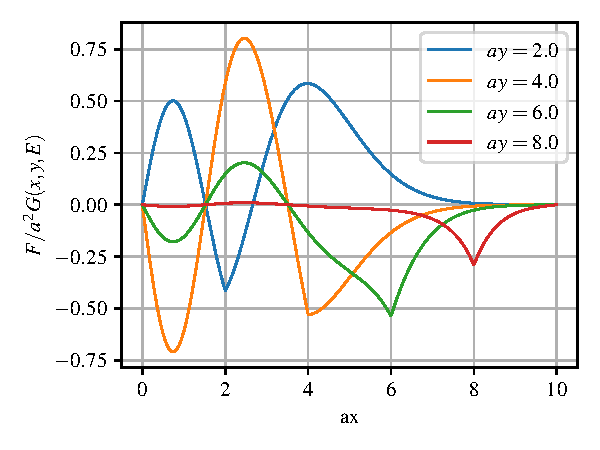
\includegraphics[scale=1]{./figs/1dgreens.pdf}
	\caption[Egy dimenziós Green-függvény]{}
	\label{egzakt:1dgreens}
\end{figure}

\begin{figure}[H]
	\centering
	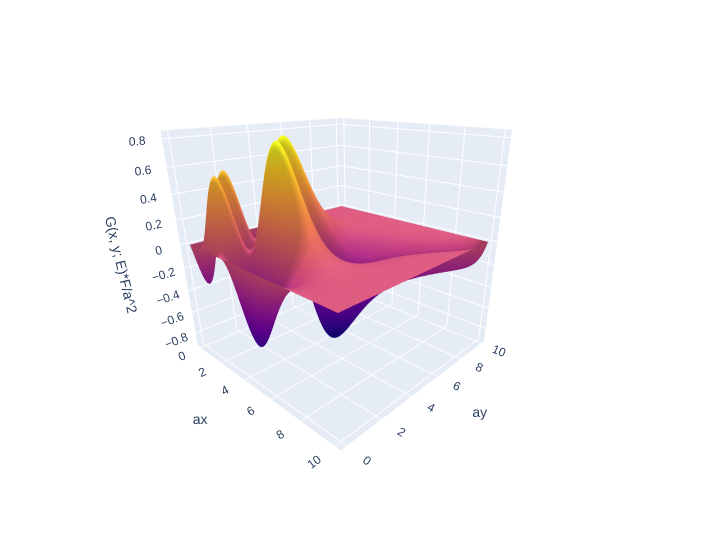
\includegraphics[scale=0.65]{./figs/2dgreen.png}
	\caption[Két dimenziós Green-függvény]{}
	\label{egzakt:2dgreen}
\end{figure}

\Aeqref{green:greensum} egyenletnek megfelelően a Green-függvénynek pólusai vannak $E=E_n$-ben. Ezt \aeqref{egzakt:greenfunction} egyértelmen mutatja, mivel a nevezőjében \aeqref{box_energiaszintek_egyenlet} $0$-ra rendezett egyenlet bal oldala szerepel. Ennek az egyenletnek a gykei határozták meg az $E_k$ sajátenergiákat.

Egy érdekes matematikai következmény, hogy a Green-függvényre vonatkozó differenciál egyenlet megoldásával elvégeztük \aref{green:greensum}. egyenlet összegzését. Ez az összeg az Airy függvények szorzatának összege lenne, osztva $E-E_k$-val és a megfelelő $N_k$ normálási faktorral ahol $E_k$-t \aeqref{box_energiaszintek_egyenlet} transzcendens egyenlet határoz meg. A Green-függvényre vonatkozó differenciálegyenlet ismerete nélkül az összeg elvégzése reménytelennek látszana.